\subsection{資料庫規劃}

本節將會介紹本系統所需之資料模型與資料庫設計概念。本系統具有兩個相對複雜且重複性高的功能:「關注」與「留言」;更甚者,此二功能都是未來有可能因為各自牽涉之主體有所異動而需要擴充的部份,因此將此二者予以抽象化就是一項重要的工作。圖~\ref{pic:data:followability} 與圖~\ref{pic:data:commentability} 分別對應上述兩項功能的抽象資料模型。可以看到兩圖的樣式非常接近,因此更進一步的抽象化是可能的。但是考量到可能之系統規模之後,為了避免過度設計 (over-design) 這邊就不予以進行更進一步之抽象化。另一方面兩圖中灰色的部份是未來可擴充之部分,但是同樣因為系統規模與時程考量而不予實作。

\begin{figure}[h]
\centering
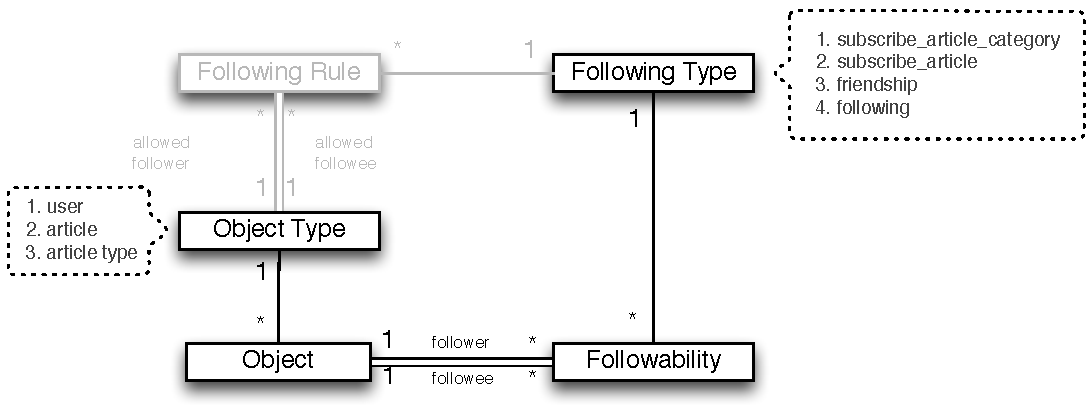
\includegraphics[width=1.05\textwidth]{img/datamodel/followability_real.pdf}
\caption{Data Model -- Followability Model}
\label{pic:data:followability}
\end{figure}

\begin{figure}[h]
\centering
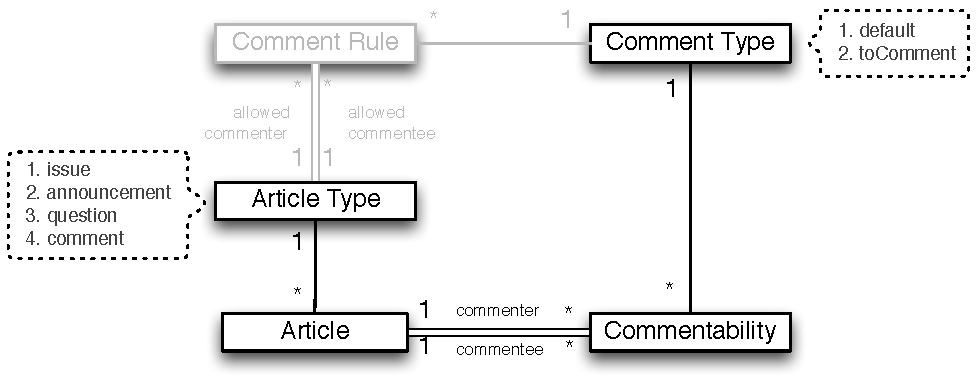
\includegraphics[width=1.05\textwidth]{img/datamodel/commentability.pdf}
\caption{Data Model -- Commentability Model}
\label{pic:data:commentability}
\end{figure}

圖~\ref{pic:data:followability} 描述了廣義的「關注」行為。此行為之概念如下:兩物件 (Object)  可以行成一組關注關係,而根據兩物件與該關注關係之種類可以決定一組實際的系統行為。此模型可以描述例如文章訂閱以及使用者關注等功能。更多「關注」相關的實際資料庫設計請參考小節~\ref{sssec:following} 與 ~\ref{sssec:subscription}。

圖~\ref{pic:data:commentability} 描述了概念性的「留言」。本系統目前僅有兩種留言模式:預設,以及巢狀留言。預設留言係指使用者可以針對所有非留言之文章進行留言,而巢狀留言則是特指針對現有之留言進行留言。留言行為本身的抽象化是為了未來文章種類或是留言相關功能之擴充所需。更多「留言」相關的實際資料庫設計請參考小節~\ref{sssec:forum}。

%% ####################### %%
\subsubsection{個人資料管理模組}
\label{sssec:userprofile}
使用者資料之資料庫模型如圖~\ref{pic:data:user} 所示,使用者資訊根據修改的程度與層級區分成三塊:
\begin{itemize}
\item 不可由個人自行更動的個人系統訊息 (users\_sysinfo)
\item 可更動之個人系統訊息 (users\_info)
\item 可更動之個人公開訊息 (users\_pubprofile)
\end{itemize}
一組使用者資訊會對應到某個使用者類別,目前預設的類別有:校友、學生、教員、職員。一組使用者資訊也會對應到一串工作經歷,而一項工作經歷會包含一項該工作期間的任職單位。任職單位的抽象化有助於未來履歷的建立與搜尋以及企業徵才的便利性。

\begin{figure}[h]
\centering
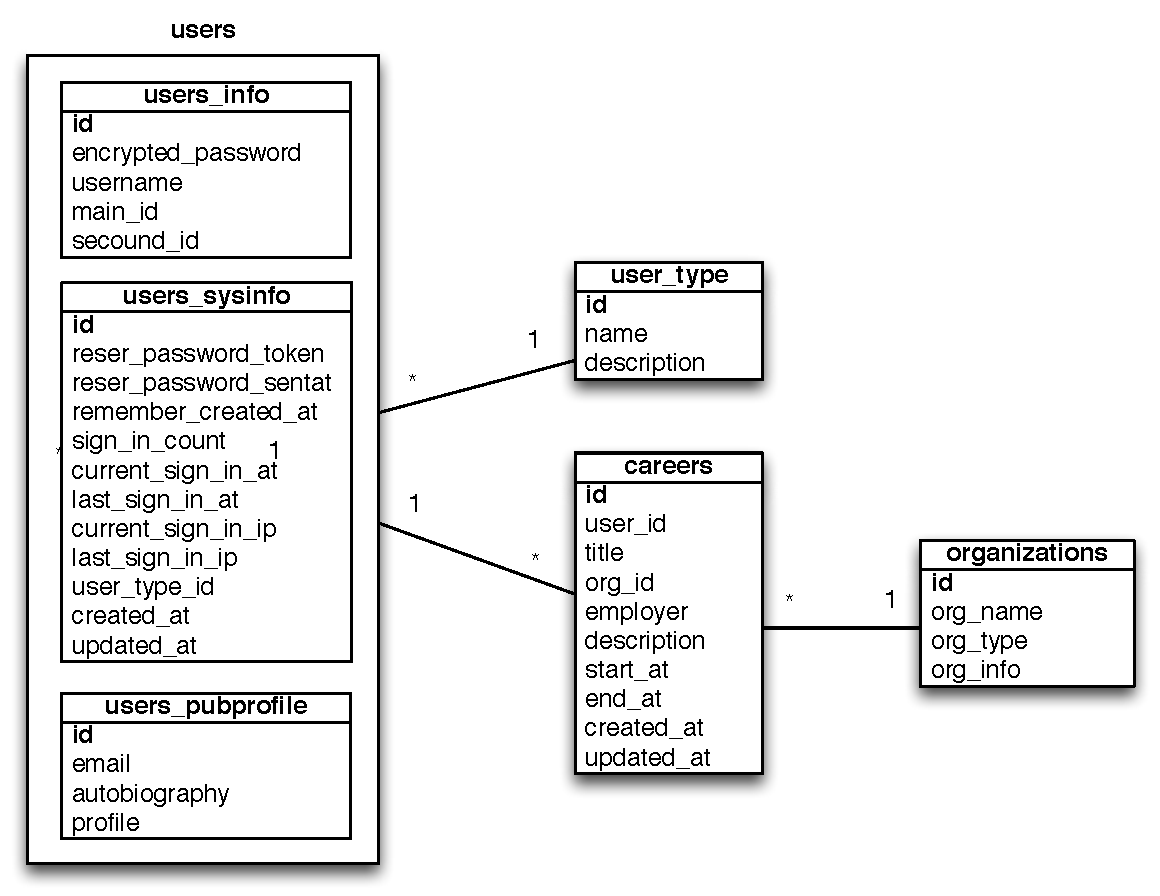
\includegraphics[width=1.05\textwidth]{img/datamodel/user.pdf}
\caption{Data Model -- User Model}
\label{pic:data:user}
\end{figure}

%% ####################### %%
\subsubsection{關係建立模組}
\label{sssec:following}
建立關係所需的資料庫模型如圖~\ref{pic:data:user2user} 所示,圖~\ref{pic:data:user2user} 中描述兩個使用者之間可以存在兩種關係:
\begin{itemize}
\item{好友 (friendship) -- 需要對方的允許、可以閱讀對方所以非公開資訊}
\item{關注 (following) -- 無需對方的允許、對方發文時會有通知信}
\end{itemize}
本模組之資料庫是實踐圖~\ref{pic:data:followability} 所描述的抽象資料模型,如是實作之價值在於保有兩使用者間的關係之可擴充性,例如說可能將完全封鎖 (Block) 給依照此模式實作成一種 Following Type 。圖~\ref{pic:data:user2user} 中兩個使用者 (user) 的實際細節請參考圖~\ref{pic:data:user}。

\begin{figure}[H]
\centering
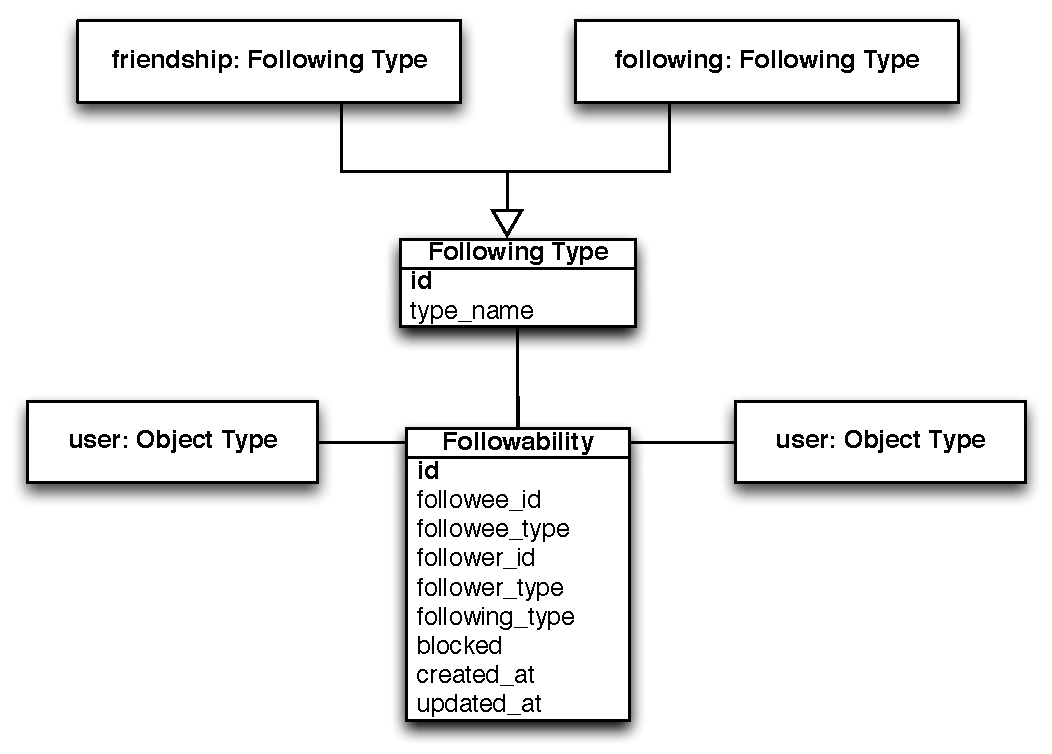
\includegraphics[width=0.85\textwidth]{img/datamodel/user2user.pdf}
\caption{Data Model -- Following and Friendship Model}
\label{pic:data:user2user}
\end{figure}

%% ####################### %%
\subsubsection{討論區模組}
\label{sssec:forum}

\begin{figure}[H]
\centering
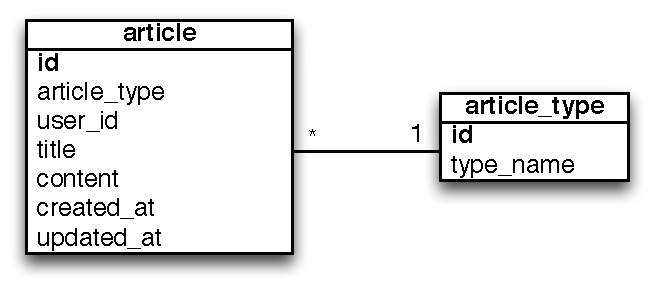
\includegraphics[width=0.6\textwidth]{img/datamodel/article.pdf}
\caption{Data Model -- Article Model}
\label{pic:data:article}
\end{figure}


討論區最基本的就是提供使用者管理文章以及發表留言等能力。文章管理,包含新增、刪除與修改等等,所需要操作之資料庫設計如下圖~\ref{pic:data:article} 所示。目前提供四種預設的文章型別:
\begin{itemize}
\item 議題 (issue) -- 一般性討論議題
\item 公告 (announcement) -- 系所或系統公告
\item 詢問 (question) -- 詢問性質之文章
\item 留言 (comment) -- 針對上述三種文章之回應
\end{itemize}

除了文章管理以外,如圖~\ref{pic:data:commentability} 所描繪之留言機制也是討論區的一個重點功能。圖~\ref{pic:data:comment2article} 意指一筆留言可以對應到一筆任意型別之文章,且根據後者個型別而有不同之行為。例如說預設的情況是:留言在非留言之文章會寄出通知信給原作者並且更新統計資訊;但若是留言給留言本身的話則僅會在寄信給原留言者。

\begin{figure}[H]
\centering
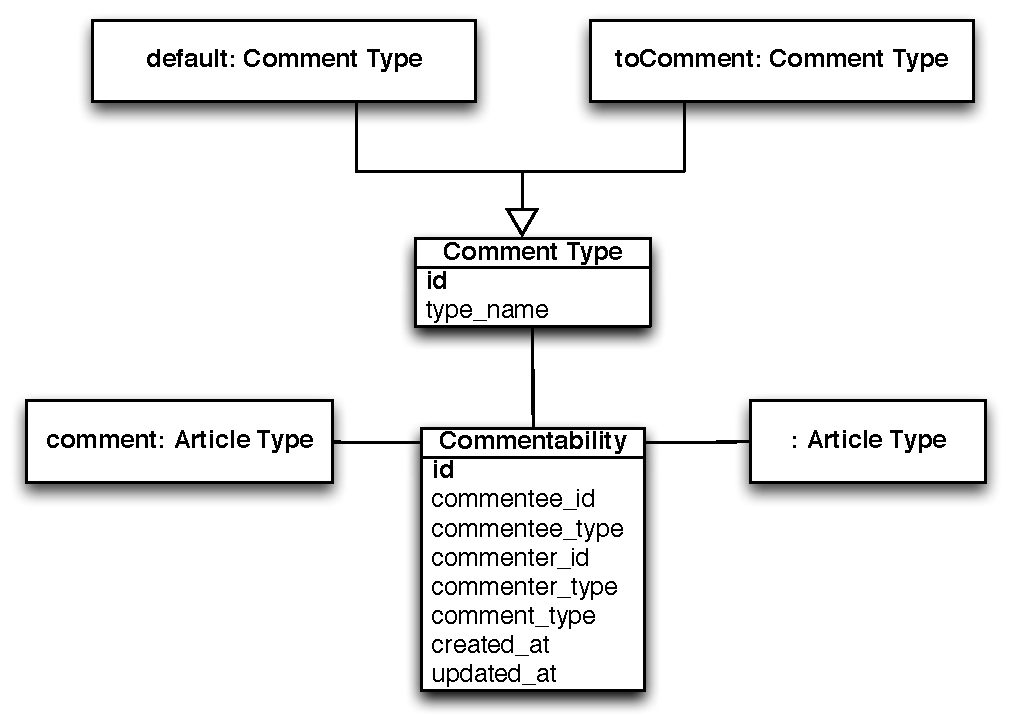
\includegraphics[width=0.85\textwidth]{img/datamodel/comment2article.pdf}
\caption{Data Model -- Comment Model}
\label{pic:data:comment2article}
\end{figure}

%% ####################### %%
\subsubsection{訂閱模組}
\label{sssec:subscription}

文章訂閱模組所需的資料庫模型如圖~\ref{pic:data:user2article} 所示,使用者可以訂閱文章 (article) 或文章類別 (article type):
\begin{itemize}
\item{訂閱文章類別 (subscribe\_article\_category) -- 有新文章時會有通知;}
\item{訂閱單一文章 (subscribe\_article) -- 有新留言時會有通知;}
\end{itemize}
本模組所需之資料庫如同小節~\ref{sssec:following} 一般,是實踐圖~\ref{pic:data:followability} 所描述之抽象資料模型。另外,圖~\ref{pic:data:user2article} 中組件如使用者 (user) 與文章 (article) 等之設計細節請參考小節~\ref{sssec:userprofile} 與~\ref{sssec:forum}。

\begin{figure}[H]
\centering
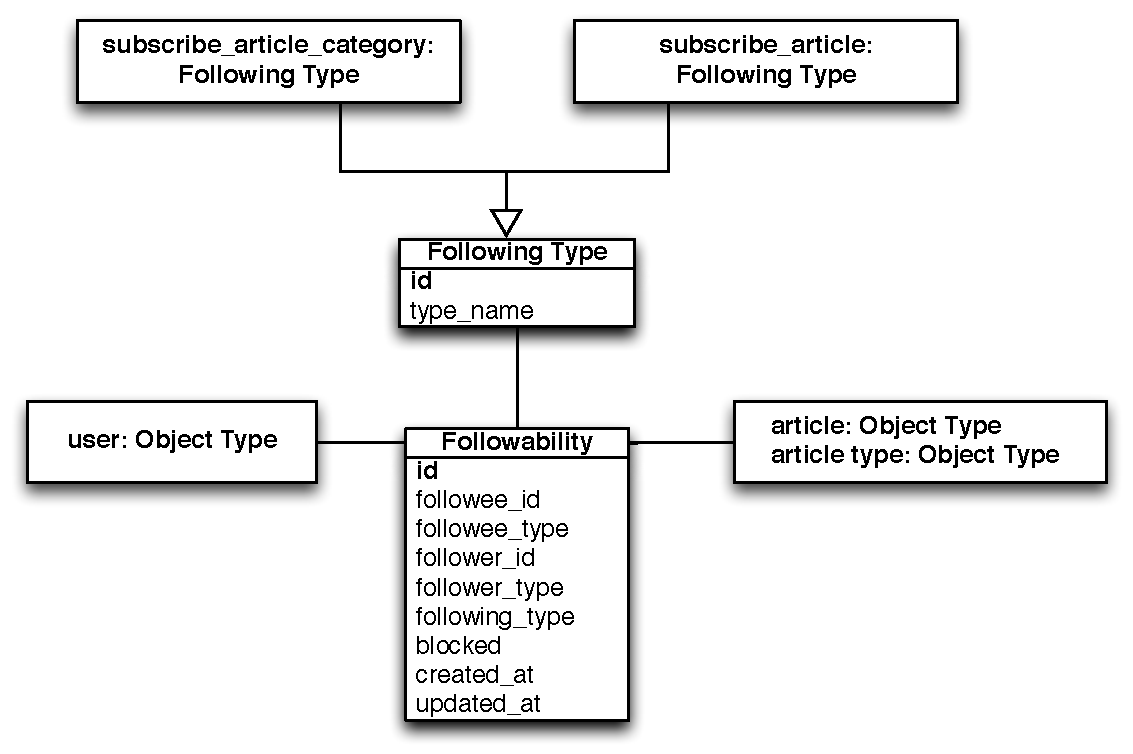
\includegraphics[width=0.85\textwidth]{img/datamodel/user2article.pdf}
\caption{Data Model -- Subscription Model}
\label{pic:data:user2article}
\end{figure}

